\documentclass[8pt]{beamer}
\usepackage[utf8]{inputenc}
\usepackage{xcolor}
\usepackage{colortbl}
\usepackage{epsfig}
% \usepackage{cancel}
\usepackage{ulem}
% \usepackage{threeparttable} % Joao Pela: 
\usepackage{amsmath}
\usepackage{hyperref}
% \usepackage{appendixnumberbeamer}
\usepackage{feynmp}         % For latex produced Feynman Diagrams

%Rule for feynmp diagrams to be considered graphics
\DeclareGraphicsRule{*}{mps}{*}{}

% New compile sequence for feynmp
\makeatletter
\def\endfmffile{%
  \fmfcmd{\p@rcent\space the end.^^J%
          end.^^J%
          endinput;}%
  \if@fmfio
    \immediate\closeout\@outfmf
  \fi
  \ifnum\pdfshellescape=\@ne
    \immediate\write18{mpost \thefmffile}%
  \fi}
\makeatother

\usetheme{Madrid}

\author[J. Pela]{João Pela}
\title{VBF Higgs to Invisible Run 2 trigger}
\institute[ICL]{Imperial College London}
\date{2014-12-04}

% The log drawn in the upper right corner.
\logo{\includegraphics[height=0.115\paperheight]{img/Logo_CMSICL.png}}

\begin{document}
\setlength{\unitlength}{1mm}

% ###################################################
\begin{frame}
  \titlepage
\end{frame}

% ###################################################
\begin{frame}{Today's presentation}
 
\begin{block}{Topics}
 
\begin{itemize}
  \item CMS Detector
  \item Legacy system
  \item Upgrade system
  \item VBF Higgs to invisible signature
  \item Designing a new trigger
\end{itemize}
 
\end{block}

\end{frame}

% ###################################################
\begin{frame}{Me @ CMS}
 
  \begin{columns}
    \column[t]{6.5cm}
    \begin{block}{Masters}

      \begin{itemize}
        \item $t\bar{t} \rightarrow b\bar{b}e\tau$ and $b\bar{b}\mu\tau$ 
        \item minimal Universal Extra Dimension $\rightarrow$ 3-4 leptons
        \item ECAL service work
      \end{itemize}

    \end{block}

    \begin{block}{CERN Engineer Internship}

     \begin{itemize}
        \item Level 1 Trigger Monitoring
      \end{itemize}

    \end{block}

  \begin{block}{PhD (3rd-ish year... not really)}

    \begin{itemize}
      \item $Higgs \rightarrow \gamma\gamma$ Spin analysis
      \item VBF $Higgs \rightarrow Invisible$
      \begin{itemize}
        \item Trigger designed (2012 and 2015)
        \item Analysis development
        \item Cross check analysis
      \end{itemize}
    \end{itemize}

  \end{block}

    \column[t]{4.5cm}
    \begin{block}

    \begin{center}
      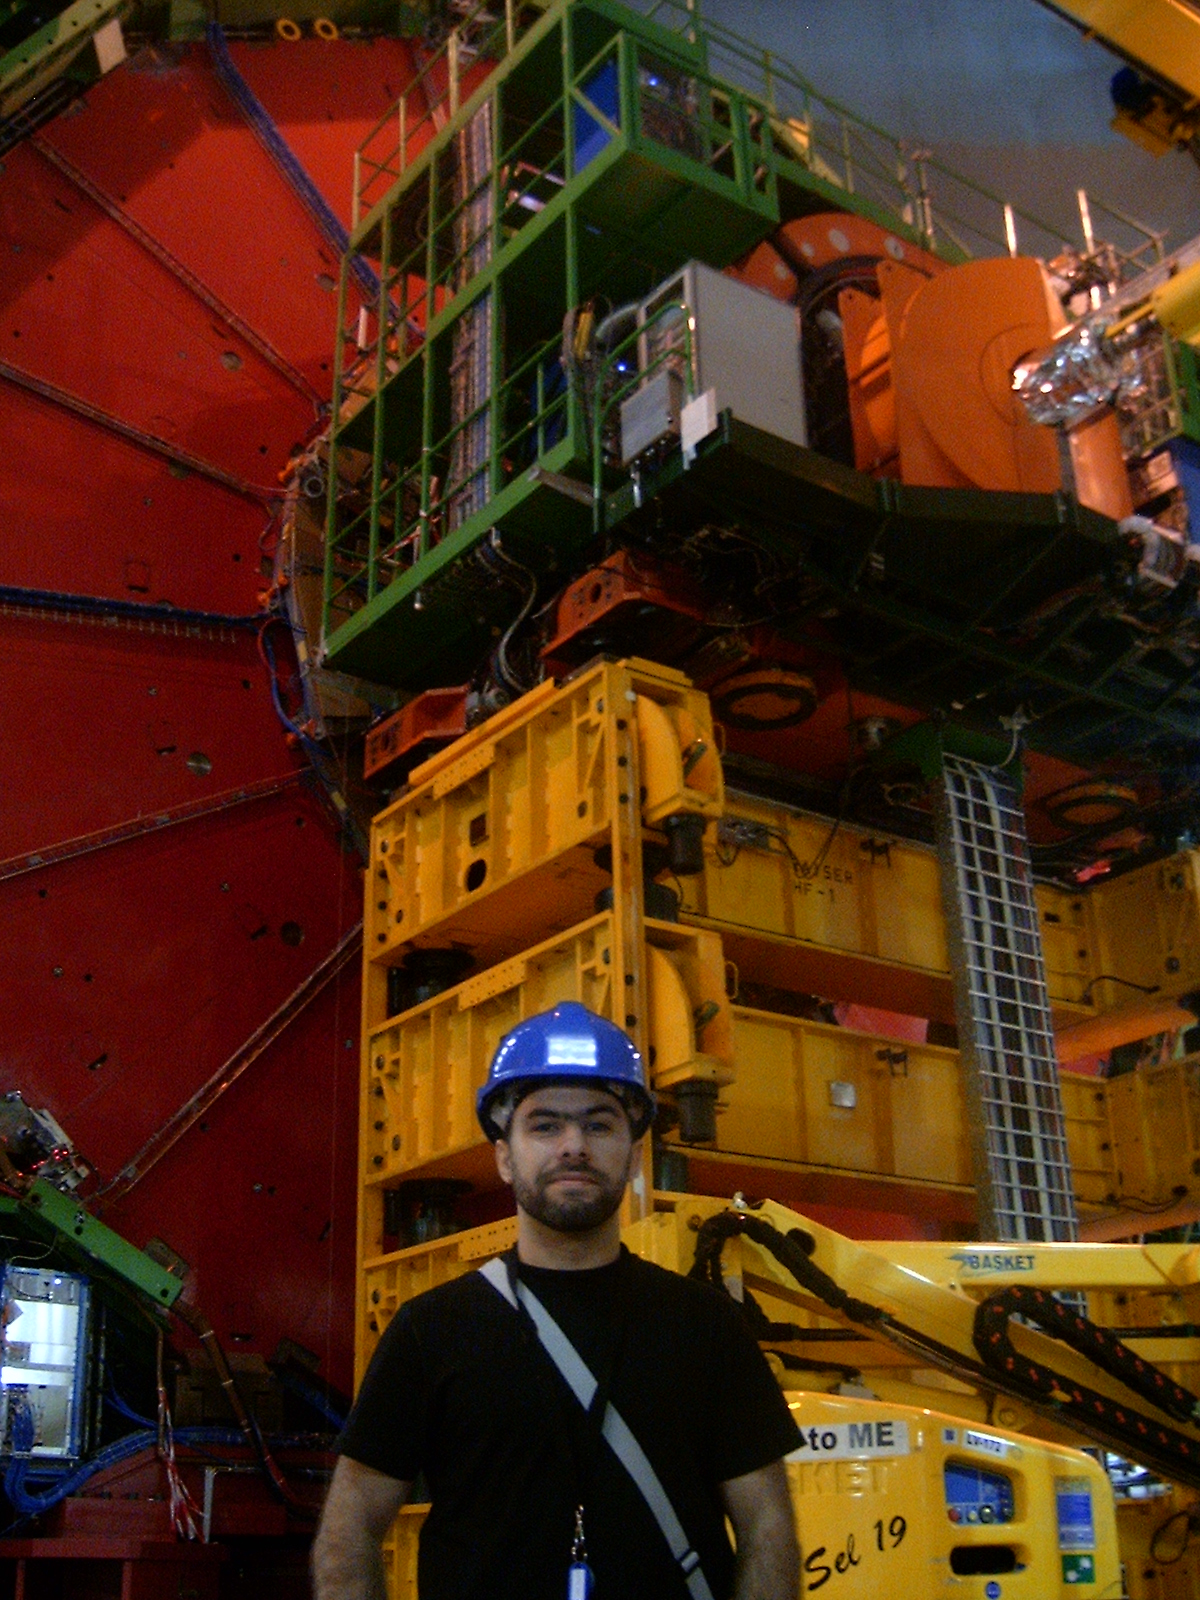
\includegraphics[width=1.00\textwidth]{img/MeAtCMS.jpg} 
    \end{center}

  \end{block}

  \end{columns}

\end{frame}

% ###################################################
\begin{frame}{The LHC-CMS Experiment}
 
  \begin{block}{Large Hadron Collider}
  
    \vspace{-5mm}
    \begin{columns}

      \column[t]{5.5cm}
      \begin{center}
        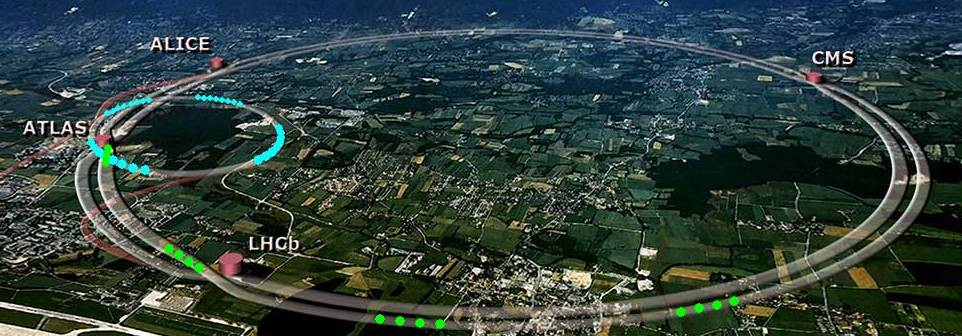
\includegraphics[width=1.00\textwidth]{img/LHCMap.jpg} 
      \end{center}

      \column[t]{5.5cm}

      \begin{itemize}
        \item Located at Franco-Swiss border near Geneva, Switzerland.
        \item Synchrotron Machine (currently the most powerful in activity)
        \item Designed to collide protons up to $\sqrt{s}=14$ $TeV$
        \begin{itemize}
          \item \tiny 2011: $\sqrt{s}=7$ $TeV$ 
          \item \tiny 2012/13: $\sqrt{s}=8$ $TeV$ 
          \item \tiny 2015: $\sqrt{s}=13$ $TeV$
        \end{itemize}
      \end{itemize}

    \end{columns}

  \end{block}

  \begin{block}{Compact Muon Solenoid}

    \vspace{-5mm}
    \begin{columns}
      \column[t]{6.5cm}

      \begin{itemize}
        \item Located at LHC Point 5
        \item General purpose experiment
        \item Objective of studying a broad spectrum of physics
        \item Classical onion structure
        \item Solenoid with highest stored energy ever built (2.66 $GJ$ at 4.0 $T$)
      \end{itemize}  

      \column[t]{4.5cm}
      \begin{center}
        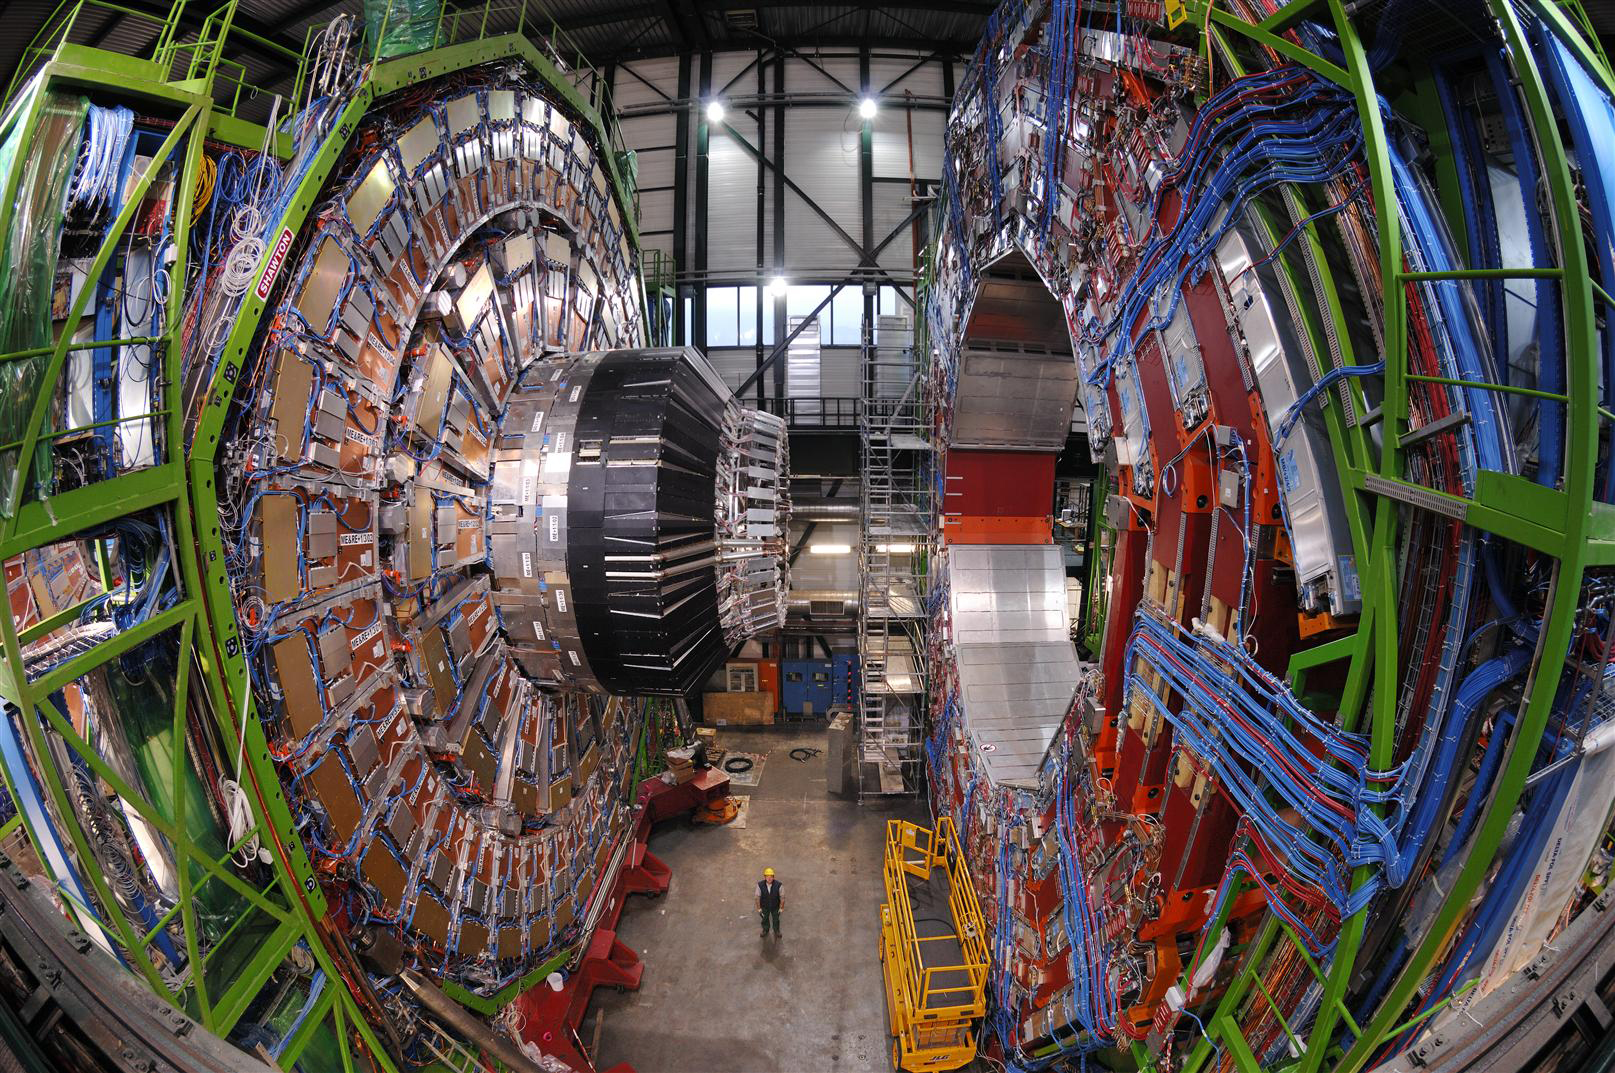
\includegraphics[width=1.00\textwidth]{img/CMSOpen.jpg} 
      \end{center}

    \end{columns}

  \end{block}

\end{frame}

% ###################################################
\begin{frame}{Particle Detection on CMS}

When a collision happens then resulting particles need to be identified and measured
 
 \begin{block}{Detector Structure}

  \begin{columns}
    \column[t]{8.0cm}
 
      \begin{center}
        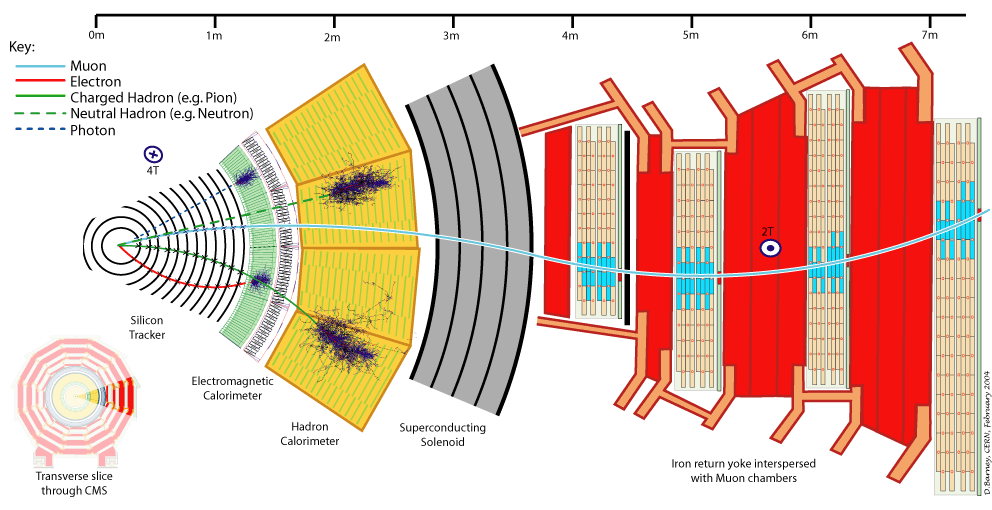
\includegraphics[width=1.00\textwidth]{img/CMS_Slice.png} 
      \end{center}  
      \column[t]{3.5cm}

       \begin{itemize}
         \item Tracker
         \begin{itemize}
           \item Charged particle trajectory
         \end{itemize}
         \item ECAL and HCAL
         \begin{itemize}
           \item Energy Measurement
         \end{itemize}
         \item Solenoid
         \begin{itemize}
           \item Charge and Momentum 
         \end{itemize} 
         \item Muon Chambers
         \begin{itemize}
           \item Muon identification and measurement 
         \end{itemize} 
         \item Trigger (L1+HLT)
         \begin{itemize}
           \item Event Selection 
         \end{itemize} 
       \end{itemize}

    \end{columns}

  \end{block}

  \begin{itemize}
    \item Detector subsystems are designed to take advantage of particle characteristics in order to identify and measure
          their characteristics.
    \item Trigger System is responsible to select only the most interesting events
  \end{itemize} 

\end{frame}

% ###################################################
\begin{frame}{CMS Trigger System Overview}

CMS has a 2 level trigger system

\begin{block}{Collisions}

At maximum operating capability during run 2 the LHC will

  \begin{itemize}
    \item Collide bunches every 25 ns
    \item Over 50 simultaneous collisions per bunch crossing
  \end{itemize}

\end{block}

\begin{block}{Level 1 Trigger}

  \begin{itemize}
    \item Hardware based system
    \item System will have to take decisions at 40 $MHz$
    \item Can only allow $\sim100$ $kHz$ events to pass
    \item Limited amount of event information and time for calculation 
  \end{itemize}

\end{block}

\begin{block}{High Level Trigger}

  \begin{itemize}
    \item Software based system (running on a CPU farm)
    \item Can only allow $\sim1$ $kHz$ events to be recorded
    \item Almost full information about the event 
  \end{itemize}

\end{block}

\end{frame}

% ###################################################
\begin{frame}{CMS Legacy L1T Trigger}
 
\begin{columns}
    
  \column[t]{5.5cm}  
  \begin{block}{Description}
 
    \begin{itemize}
      \item Calorimeter data e gathered into regions
      \item Muon segment are found (taking system overlap into account)
      \item Global calorimiter objects and sums are computed
      \item Global muon information is merged
      \item Global trigger evaluates algorithms
      \item Final decision is sent back to detector and DAQ
    \end{itemize}
   
  \end{block}
   
  \column[t]{5.5cm}
  \begin{block}{Diagram} 
  
    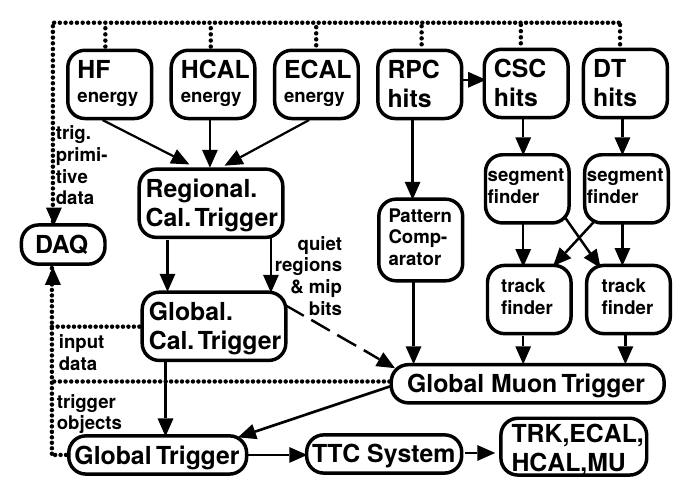
\includegraphics[width=1.00\textwidth]{img/L1TLegacyDiagram.png} 
 
  \end{block}

\end{columns}

\end{frame}

% ###################################################
\begin{frame}{CMS Upgrade System Trigger}

Besides more $\sqrt{s}$ energy in run 2 we will almost double the number of interaction per bunch crossing and double the crossing rate. Legacy still will struggle to deal with this. We need a new Level 1 trigger!

\begin{columns}
    
  \column[t]{5.5cm}  
  \begin{block}{Description}
   
  \begin{itemize}
    \item No regional calorimeter data gathering
    \item No system specific track searching
    \item Global calorimeter object and sum calculation
    \item Global (by region) muon track finding
    \item Calorimeter information is shared with muon (for isolation calculation)
    \item Global trigger evaluates algorithms
    \item Final decision is sent back to detector and DAQ
  \end{itemize}

  \end{block}

  \column[t]{5.5cm}
  \begin{block}{Diagram} 
  
    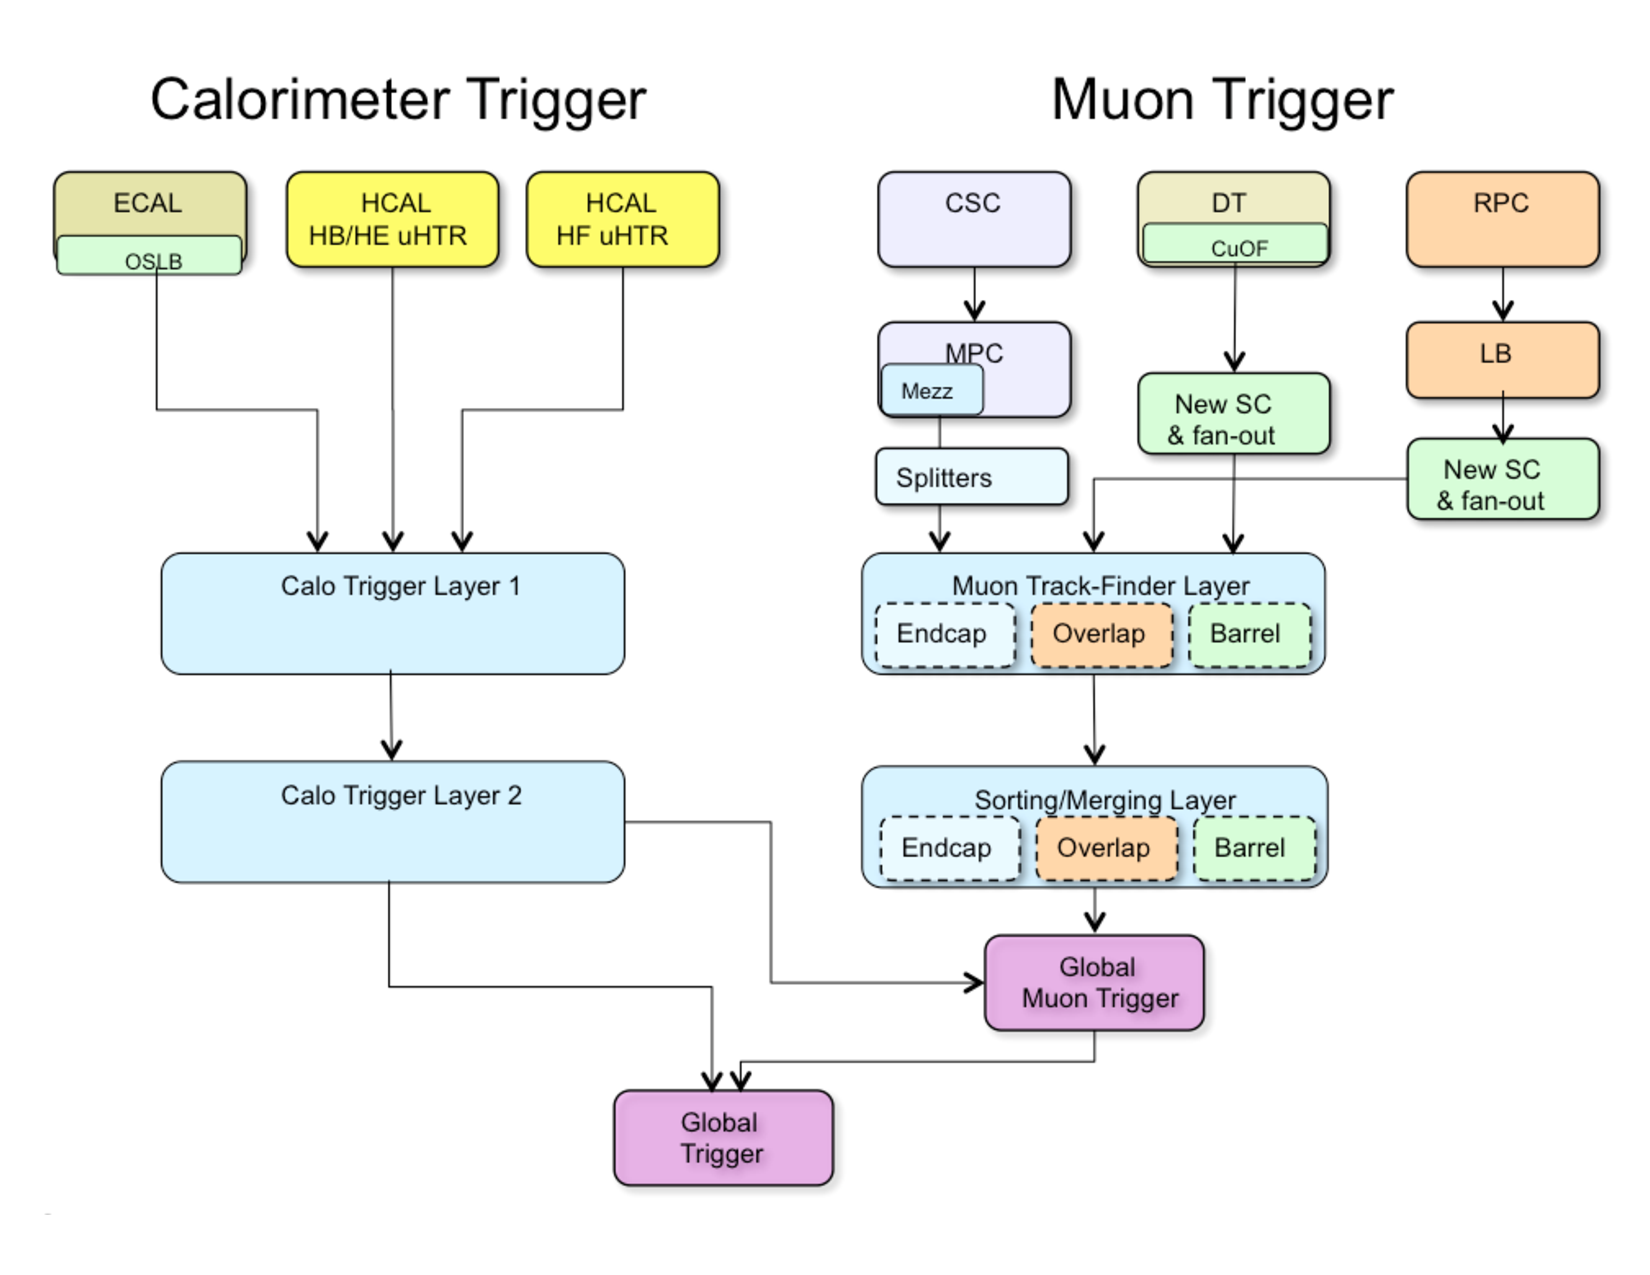
\includegraphics[width=1.00\textwidth]{img/TrigUpgradeBlockDiagram} 
 
  \end{block}

\end{columns}
 
Also we are implementing a new global architecture for the whole L1T. Instead of processing events linearly event by event they will be time multiplexed over several cards each with full access to all event information. 

\end{frame}

% ###################################################
\begin{frame}{New L1T possibilities}
 
\begin{block}{Hardware:}

\begin{itemize}
  \item More flexibility
  \begin{itemize}
    \item Large FPGA and memory resources
    \item Higher bandwidth via optical links
  \end{itemize}
  \item Less card diversity (small number of general-purpose cards)
  \item Upgrade system will run in parallel with legacy system (at least initially)
\end{itemize}

 
\end{block}

\begin{block}{Algorithms:}

\begin{itemize}
  \item PU subtraction
  \item Better jet position and energy resolution
  \item Incorporation of forward jets from HF (important)
  \item Possible inclusion of HF in energy sums (important for MET)
  \item Much better $\tau$ identification
  \item Isolated Muon Isolation algorithms (Additional system interconnection)
  \item Possibility of more complex calculations at L1T:
  \begin{itemize}
    \item Invariant Mass triggers
    \item Better b-tagging of jets (jets with a muon)
    \item Angular separation ($\Delta\eta$, $\Delta\phi$, etc)
    \item Other advanced algorithms (your idea can be here!)
  \end{itemize}
\end{itemize}

\end{block}

\end{frame}

% ###################################################
\begin{frame}{Lowest seeds}

The beam conditions are $\sqrt{s}=14$ TeV and $L=2.2 \times 10^{34}~{\rm cm^{-2}s^{-1}}$ with a bunch spacing of 25 ns and pile-up of 50
   
\begin{block}{Seeds}

\centering
\resizebox{0.7\linewidth}{!}{
\begin{tabular}{|l|c|c|c||c|c|c|} 
\hline
& \multicolumn{3}{c||}{Current Level-1} & \multicolumn{3}{c|}{Upgraded Level-1} \\
& \multicolumn{3}{c||}{$L=2.2 \times 10^{34}~{\rm cm^{-2}s^{-1}}$} & \multicolumn{3}{c|}{$L=2.2 \times 10^{34}~{\rm cm^{-2}s^{-1}}$} \\			
\hline
&	     &     95\%      	&           &      &    95\% &       \\
Trigger& Rate &      Threshold        & Plateau   & Rate &      Threshold        & Plateau \\
Algorithm& [kHz]&     [GeV]  & Efficiency & [kHz]&     [GeV]& Efficiency \\        
\hline\hline  
Single e/$\gamma$ 	  &  10  &    67  	 & 1.0  &  11   &  57		& 1.0  \\ %1.0 				%selection: all EG all eta
\hline  Single iso e/$\gamma$&  9.4 &    52  	 & 0.9  &  15   &  31		& 0.90 \\ %0.9 				%selection: eta<2.17
\hline  Single Mu   		     &  11  &    42  	 & 0.95 &  14   &  22		& 0.90 \\ %0.95				%selection: eta<2.1 Qual>=4
\hline  Single iso Mu   	  &	NA &    NA  	 &  NA  &  15   &  19		& 0.82 \\ % NA 				%selection: eta<2.1 Qual>=4
\hline  Single Tau			  &	NA &    NA  	 &  NA  &  12   & 100		& 0.95 \\ %0.6 				%selection: eta<2.17
\hline  Single iso Tau		  &  9.2  & 	72 	 & 0.3  &  13   &  83		& 0.7  \\ % NA 			%selection: eta<2.17 	  
\hline  iso e/$\gamma$ + e/$\gamma$	  & 16   &    26   16 & 0.9  &  12   &  23	16 & 0.9   \\ %1.0$\times$1.0   %selection: all EG all eta
\hline  (iso)Mu + Mu 		  &  7.4 &    20   12 & 0.9  &	9.4 &  15	10 & 0.8 \\ %0.95$\times$0.95  %selection: Qual>=4
\hline  (iso)Tau + Tau  	  &  8.2 &    36   36 & 0.1  &	7.2 &  64	62 & 0.67 \\ %0.6$\times$0.6 %selection: eta<2.17
\hline  iso e/$\gamma$ + Mu  &  6.2 &    24   12 & 0.85 &  11   &  21	10 & 0.85 \\ %1.0$\times$0.95  %selection: qual>=4 relative cuts??
\hline  (iso)Mu + e/$\gamma$ &  5.0 &    20   15 & 0.95 &	8.3 &  18	15 & 0.83 \\ %0.95$\times$1.0  %selection: qual>=4 relative cuts??
\hline  iso e/$\gamma$ + Tau &	NA &  	 NA	 &  NA  &	8.3 &  21	57 & 0.86 \\ %1.0$\times$0.6 %selection:
\hline  isoMu + Tau  		  &	NA &  	 NA	 &  NA  &	5.8 &  14	47 & 0.8  \\ %0.95$\times$0.6  %selection: qual>=4
\hline  Single Jet			  &  5.4 &   205  	 & 1.0  &	5.9 & 205		& 1.0  \\ %1.0 				%selection: central jets
\hline  Double Jet			  &  5.8 &   170  170 & 1.0  &	4.2 & 130  130 & 1.0  \\ %1.0 				%selection: Only Central Jets
\hline  Quad Jet  			  &  4.8 &   4@96 	 & 1.0  &	5.0 &  4@55 	& 1.0  \\ %1.0 				%selection: only Central jet (no tau!)
%			\hline  Six Jet				  &  5	& 3@120  3@81& 1.0  &	3.0 & 3@55 3@43& 1.0  \\ %1.0 				%selection: central jets
\hline  Single iso e/$\gamma$ +  Jet  &  8.5 &    38   82 & 0.9  &  11   &  27	78 & 0.90 \\ %0.9$\times$1.0    %selection: eta<2.17
\hline  Single Mu +  Jet	  &  7.5 &    27   54 & 0.95 &	9.7 &  18	52 & 0.93 \\ %0.95$\times$1.0   %selection: eta<2.1 Qual>=4
\hline  Single iso e/$\gamma$ + $H_T^miss$&  8.2 &    38  120 & 0.9  &  12   &  27  110 & 0.90 \\ %0.9$\times$1.0    %selection: eta<2.17
\hline  Single Mu + $H_T^miss$   & 9.8  &    20   93 & 0.95 &  11   &  18	86 & 0.93 \\ %0.95$\times$1.0   %selection: eta<2.1 Qual>=4
%			\hline  $\mht$ 				  & 6.9  &    200 	 & 1.0  &	6.9  &	 200  & 1.0  \\ %1.0 				%selection: 
\hline  $H_T$ 				  & 5.4  &    580 	 & 1.0  &	3.0 & 380		& 1.0  \\ %1.0 				%selection: 						 
\hline\hline Total Rate            &  92  &  			 & 	  &	95 	 & 			 &   \\ 
\hline 
\end{tabular}
}
 
\end{block}

\end{frame}

% ###################################################
\begin{frame}{VBF Higgs to invisible and the Trigger}
 
\begin{columns}
 
  \column[t]{5.5cm}  
  \begin{block}{Feynman Diagram}
   
   \begin{fmffile}{feynmanDiagram_VBFHiggs}
  \fmfframe(0,5)(0,5){
  \begin{fmfgraph*}(40,20)
    \fmfleft{P1,P2} \fmfright{P1',H',P2'}
    \fmf{fermion}{P1,g1}
    \fmf{fermion}{P2,g2}
    \fmf{boson,label=$W/Z^0$,label.side=left}{g1,H}
    \fmf{boson,label=$W/Z^0$,label.side=left}{H,g2}
    \fmfdot{H,g1,g1}
    \fmf{boson,tension=0.2}{H,H'}
    \fmf{fermion}{g1,P1'}
    \fmf{fermion}{g2,P2'}
    \fmflabel{$H^0$}{H'}
    \fmflabel{$q_1$}{P1}
    \fmflabel{$q_2$}{P2}
    \fmflabel{$q_1'$}{P1'}
    \fmflabel{$q_2'$}{P2'}
  \end{fmfgraph*}
  }
\end{fmffile}
   
  \end{block}
    
  \begin{block}{Signature}
    
    \begin{itemize}
      \item 2 Forward jets with high dijet mass
      \item No color connection so no activity between jets
      \item Missing transverse energy
    \end{itemize}
   
  \end{block}
    
  \column[t]{5.5cm}  

  \begin{block}{Problems}

    \begin{itemize}
      \item Hadron colliders are jet factories... its easy to find 2 of them
      \item Some processes produce real MET (like b, W or Z decays)
      \item Miss measuring jets can create fake MET
      \item Detector effects like zero suppression can cause fake MET too
      \item Pile-up will provide more jets and create more complication to isolate signal
    \end{itemize}
  
  \end{block}


\end{columns}

\end{frame}

% ###################################################
\begin{frame}{Searching for a new trigger}
 
\begin{block}{Method for L1T}

Monte Carlo samples where generated to simulate just overlapped minimum bias events (with no hard scattering)

\begin{itemize}
  \item Sample replicate 3 possible scenarios of bunch separation and PU (up to 25 ns and PU 40) 
  \item We can simulate the L1T upgrade system performance
  \item We can produced L1T objects to study and emulate new algorithms
\end{itemize}
 
\end{block}

\begin{block}{Method for HLT}

We cannot use the same samples as the ones used for the L1T studies (simply not enough statistics) we use
QCD samples since this will be the dominant type of events passing any HLT trigger. 

\begin{itemize}
  \item Same 3 possible scenarios as before
  \item We can simulate the L1T+HLT upgrade system performance
  \item We start by requiring a specific L1T seed
  \item We can produced HLT objects to study and emulate new algorithms
\end{itemize}

\end{block}

For both L1T and HLT studies we used a grid search over several variables to meet specific rate and
efficiency requirements.

\end{frame}

% ###################################################
\begin{frame}{Baseline I}
 
\begin{block}{2012 Trigger}
 
\begin{itemize}
  \item L1T Seed: L1\_ETM40
  \item HLT Path: HLT\_DiPFJet40\_PFMETnoMu65\_MJJ800VBF\_AllJets\_v*
  \begin{itemize}
    \item Dijet $p_T>40$ $GeV$, fwd/bck, $\Delta\eta>3.5$, $m_{jj}>800$ $GeV$
    \item METNoMu $>65$ $GeV$
  \end{itemize}  
\end{itemize}
 
Efficiency for $m_{H}=125$, BF(Inv)=100\%, $L1_{eff}=\sim47\%$, $HLT_{eff}=\sim9\%$
 
\end{block}

We start from the baseline L1T trigger and run grid search also run some proposals from other groups.

\begin{block}{L1T for Run 2}
 
\centering
\begin{tabular}{|l|c|c|c|}
\hline
Algo & Ind. Rate & Ind. Eff. & Extra Yield \\
\hline\hline
ETM70 (on the menu) & 7 $kHz$ & 28\% & - \\
\hline\hline
$Dijet30 + fwd/bck + \Delta\eta(jj)>3.5 + Jet96$ & 4.6 $kHz$ & 15\% & 21\% \\
$Dijet30 + fwd/bck + \Delta\eta(jj)>3.5 + ETM50$ & 5.0 $kHz$ & 14\% & 14\% \\
\hline\hline
$ETM60$ + jet veto($p_T>40$ $GeV$,$\Delta\phi<1.0$) & 5.5 $kHz$ & 14\% & 11\% \\
$HTT70$ + $MHT/HTT>0.7$ & 9 $kHz$ & 22\% & 11\% \\
\hline
\end{tabular}
 
\end{block}

The baseline trigger ETM70 give us 28\% but we found 2 more trigger that will increase the yield of signal by at least 14\%. Proposals from other groups do worst.

\end{frame}

% ###################################################
\begin{frame}{Baseline II}
 
For now we will use L1T\_ETM70 as seed and see if we can design a a good baseline HLT path on top.
\begin{itemize}
  \item We need have a baseline HLT trigger HLT\_PFMET170\_NoiseCleaned
  \item Define additional HLT trigger with at most 5 $Hz$ rate
  \item Define a prescaled control trigger (for systematics) with lower MET cuts.
\end{itemize}
 
\begin{block}{HLT for Run 2}

Again we run the grid search but for HLT variables

\centering
\resizebox{1.0\linewidth}{!}{
\begin{tabular}{|l|c|c|c|c|}
\hline
HLT Path & L1 Seed & Rate & Eff. & Total eff. \\
\hline\hline
HLT\_PFMET170\_NoiseCleaned & L1\_ETM70 & - & 9\% & 9\% \\
\hline\hline
HLT\_DiPFJetVBF40\_DEta3p5\_MJJ600\_PFMETNoMu140    & L1\_ETM70 & 4.7 $Hz$ & - & 10.5\% \\
HLT\_DiPFJetVBF60-40\_DEta3p5\_MJJ600\_PFMETNoMu140 & L1\_ETM70 & 4.5 $Hz$ & - & 10.5\% \\
\hline\hline
Control trigger & & & & \\
HLT\_DiPFJetVBF40\_DEta3p5\_MJJ600\_PFMETNoMu80 & L1\_ETM50 & 0.5 $Hz$ & - & - \\
\hline
\end{tabular}
}

\end{block}

We have found 2 HLT paths that will increase signal yield by by over 25\% using also L1\_ETM70 as seed. This paths are now included on the menu for MC production and will be used for data recording (if not improved until then).

\end{frame}

% ###################################################
\begin{frame}{Summary}
 
\begin{block}{Summary:}
 
\begin{itemize}
  \item The starting point for any analysis is designing (or selecting) an appropriate trigger.
  \item Knowing the topology of your signal and detector/trigger capabilities is essential
  \item We were able to design a new baseline Run II trigger for VBF Higgs to Invisible which not only keep but increases signal efficiency
        compared with 2012.
  \item Studies are ongoing to improve baseline by reducing thresholds and adding extra conditions.
\end{itemize}

\end{block}

\end{frame}

\end{document}